\documentclass[a4paper,12pt]{article}
\usepackage{xcolor}
\usepackage{algorithm}
\usepackage{algorithm}
\usepackage{algpseudocode}
\usepackage{amsmath,amsfonts,amssymb}
\usepackage{geometry}
\usepackage{fancyhdr}
\usepackage{graphicx}
\usepackage{subcaption}
\usepackage{caption}
\usepackage{titlesec}
\usepackage{tikz}
\usepackage{booktabs}
\usepackage{array}
\usetikzlibrary{positioning,arrows.meta} % Load the positioning library

\usetikzlibrary{shadows}
\usepackage{tcolorbox}
\usepackage{float}
\usepackage{lipsum}
\usepackage{mdframed}
\usepackage{pagecolor}
\usepackage{mathpazo}   % Palatino font (serif)
\usepackage{microtype}  % Better typography

% Page background color
\pagecolor{gray!10!white}

% Geometry settings
\geometry{margin=0.5in}
\pagestyle{fancy}
\fancyhf{}

% Fancy header and footer
\fancyhead[C]{\textbf{\color{blue!80}CS726 Programming Assignment -- 2 Report}}
\fancyhead[R]{\color{blue!80}Bayesian Bunch}
\fancyfoot[C]{\thepage}

% Custom Section Color and Format with Sans-serif font
\titleformat{\section}
{\sffamily\color{purple!90!black}\normalfont\Large\bfseries}
{\thesection}{1em}{}

% Custom subsection format
\titleformat{\subsection}
{\sffamily\color{cyan!80!black}\normalfont\large\bfseries}
{\thesubsection}{1em}{}

% Stylish Title with TikZ (Enhanced with gradient)
\newcommand{\cooltitle}[1]{%
  \begin{tikzpicture}
    \node[fill=blue!20,rounded corners=10pt,inner sep=12pt, drop shadow, top color=blue!50, bottom color=blue!30] (box)
    {\Huge \bfseries \color{black} #1};
  \end{tikzpicture}
}
\usepackage{float} % Add this package

\newenvironment{solution}[2][]{%
    \begin{mdframed}[linecolor=blue!70!black, linewidth=2pt, roundcorner=10pt, backgroundcolor=yellow!10!white, skipabove=12pt, skipbelow=12pt]%
        \textbf{\large #2}
        \par\noindent\rule{\textwidth}{0.4pt}
}{
    \end{mdframed}
}

% Document title
\title{\cooltitle{CS726 Programming Assignment -- 2 Report}}
\author{
\textbf{Saksham Rathi (22B1003)}\\
\textbf{Sharvanee Sonawane (22B0943)}\\
\textbf{Deeksha Dhiwakar (22B0988)}\\
\small Department of Computer Science, \\
Indian Institute of Technology Bombay \\}
\date{}

\begin{document}
\maketitle

\section*{Denoising Diffusion Probabilistic Models}

Here are the results of unconditional DDPMs on various datasets (with respect to the number of time steps). We had fixed all other parameters (the best settings observed):

\begin{itemize}
  \item lbeta=0.0001
  \item ubeta=0.02
  \item lr=0.0001 (so that training loss decreases across epochs)
  \item n\_samples=10000
  \item n\_dim=2 (for helix it is 3)
  \item batch\_size=128 (to avoid CUDA memory errors and produce optimal results)
  \item epochs=40
\end{itemize}

\clearpage
\subsection*{Moons}

\begin{figure}[H]
  \centering
  \begin{minipage}{0.3\textwidth}
      \centering
      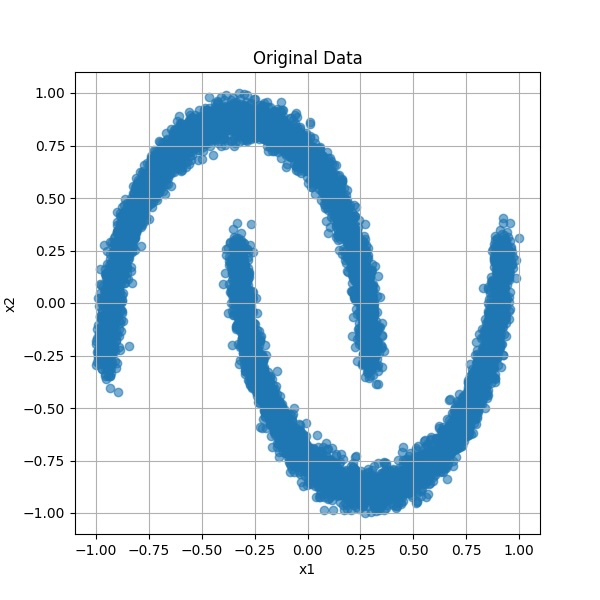
\includegraphics[width=\linewidth]{images/moon.jpg}
      \subcaption{Original Moons Dataset}
  \end{minipage}
  \begin{minipage}{0.3\textwidth}
      \centering
      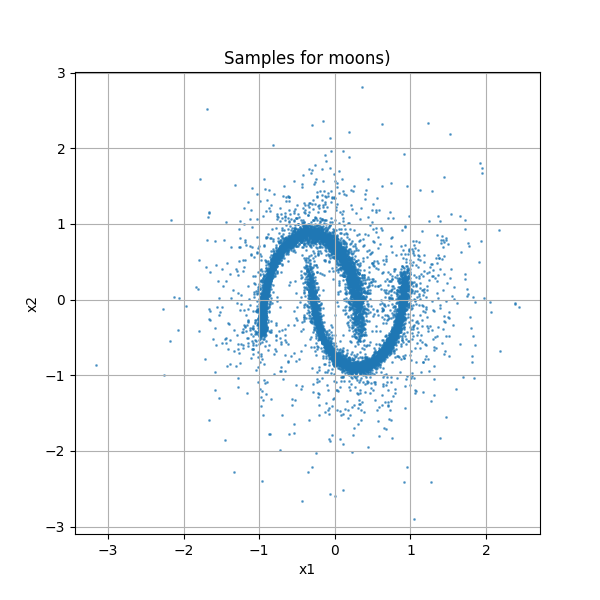
\includegraphics[width=\linewidth]{"images/Samples for ddpm_2_10_0.0001_0.02_moons.png"}
      \subcaption{Number of time steps = 10}
  \end{minipage}
  \begin{minipage}{0.3\textwidth}
      \centering
      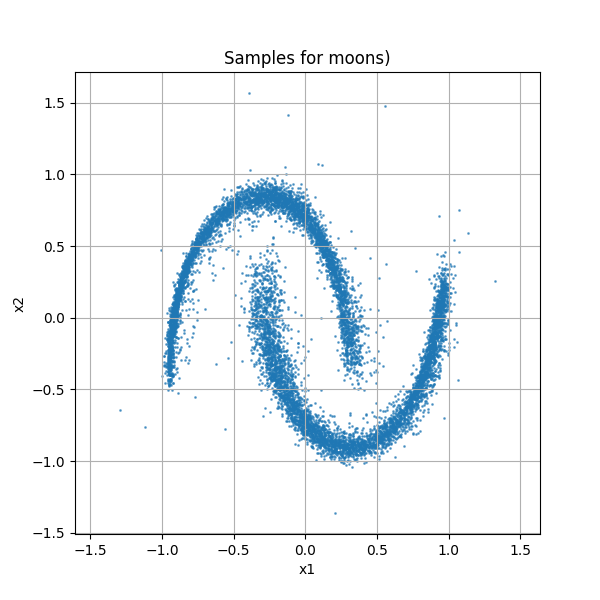
\includegraphics[width=\linewidth]{"images/Samples for ddpm_2_50_0.0001_0.02_moons.png"}
      \subcaption{Number of time steps = 50}
  \end{minipage}

  \vspace{0.5cm}

  \begin{minipage}{0.3\textwidth}
      \centering
      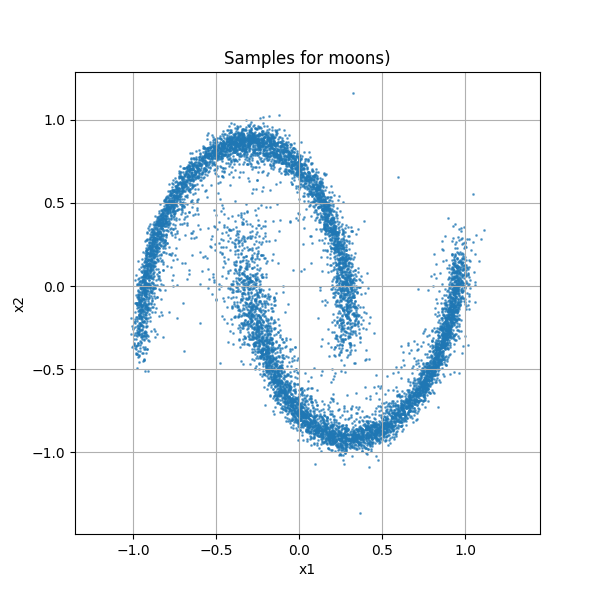
\includegraphics[width=\linewidth]{"images/Samples for ddpm_2_100_0.0001_0.02_moons.png"}
      \subcaption{Number of time steps = 100}
  \end{minipage}
  \begin{minipage}{0.3\textwidth}
      \centering
      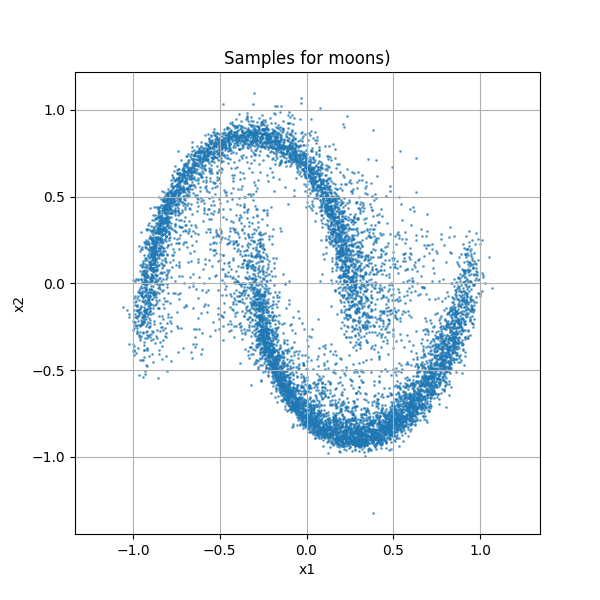
\includegraphics[width=\linewidth]{"images/Samples for ddpm_2_150_0.0001_0.02_moons.png"}
      \subcaption{Number of time steps = 150}
  \end{minipage}
  \begin{minipage}{0.3\textwidth}
      \centering
      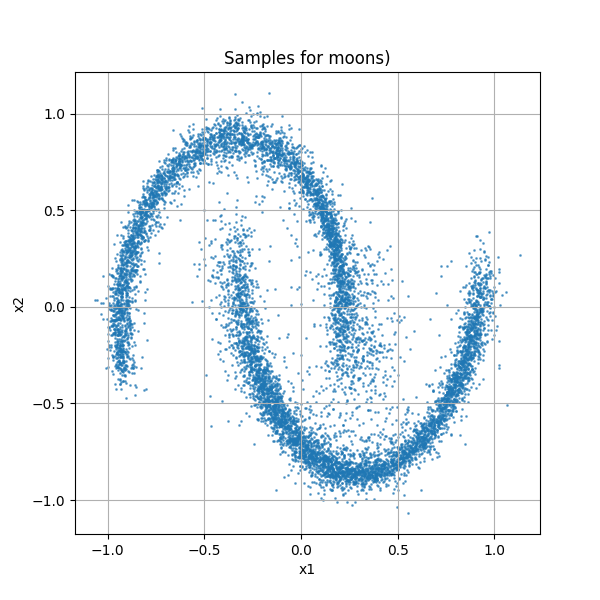
\includegraphics[width=\linewidth]{"images/Samples for ddpm_2_200_0.0001_0.02_moons.png"}
    \subcaption{Number of time steps = 200}
  \end{minipage}

  \caption{Moons Dataset}
\end{figure}

Here are the NLL values:
\begin{itemize}
  \item $T = 10$: 1.048
  \item $T = 50$: 0.9599
  \item $T = 100$: 0.9519
  \item $T = 150$: 0.9218
  \item $T = 200$: 0.9321
\end{itemize}

As, we can see from both NLL values and the images, $T = 150$ performed the best.

\clearpage



\subsection*{Blobs}

\begin{figure}[H]
  \centering
  \begin{minipage}{0.3\textwidth}
      \centering
      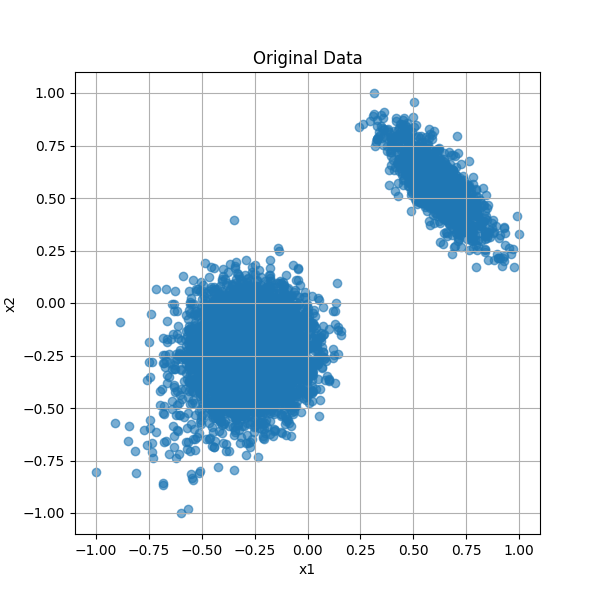
\includegraphics[width=\linewidth]{images/blobs.png}
      \subcaption{Original Blobs Dataset}
  \end{minipage}
  \begin{minipage}{0.3\textwidth}
      \centering
      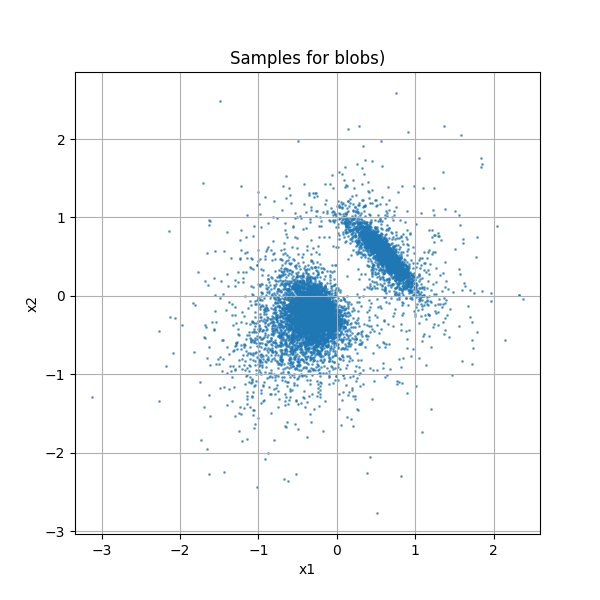
\includegraphics[width=\linewidth]{"images/Samples for ddpm_2_10_0.0001_0.02_blobs.png"}
      \subcaption{Number of time steps = 10}
  \end{minipage}
  \begin{minipage}{0.3\textwidth}
      \centering
      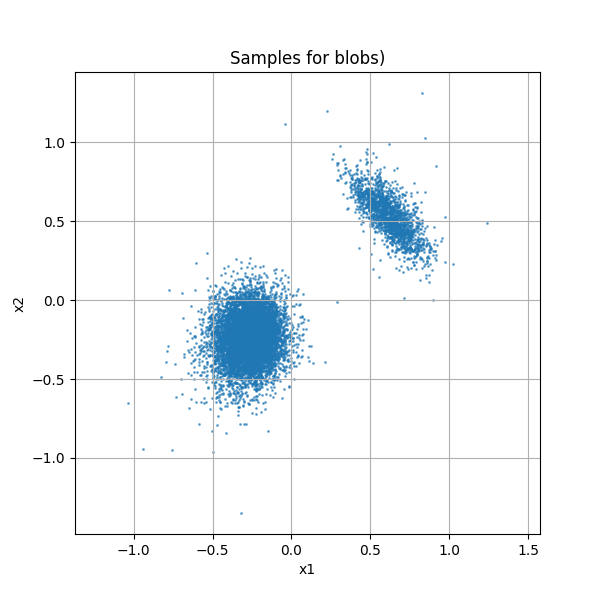
\includegraphics[width=\linewidth]{"images/Samples for ddpm_2_50_0.0001_0.02_blobs.png"}
      \subcaption{Number of time steps = 50}
  \end{minipage}

  \vspace{0.5cm}

  \begin{minipage}{0.3\textwidth}
      \centering
      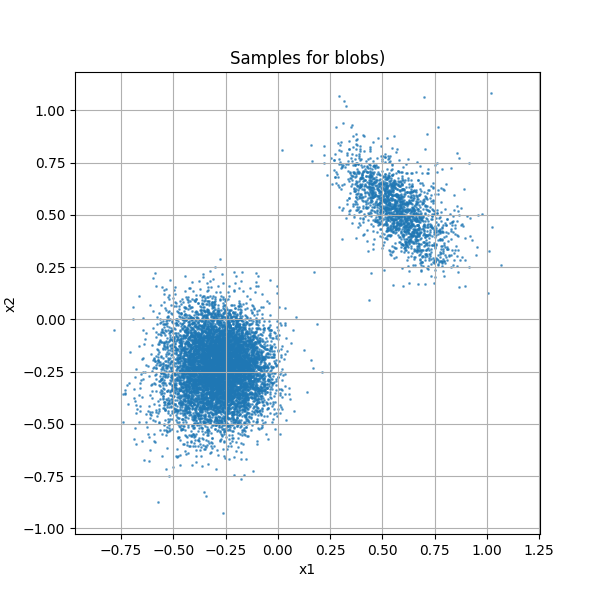
\includegraphics[width=\linewidth]{"images/Samples for ddpm_2_100_0.0001_0.02_blobs.png"}
      \subcaption{Number of time steps = 100}
  \end{minipage}
  \begin{minipage}{0.3\textwidth}
      \centering
      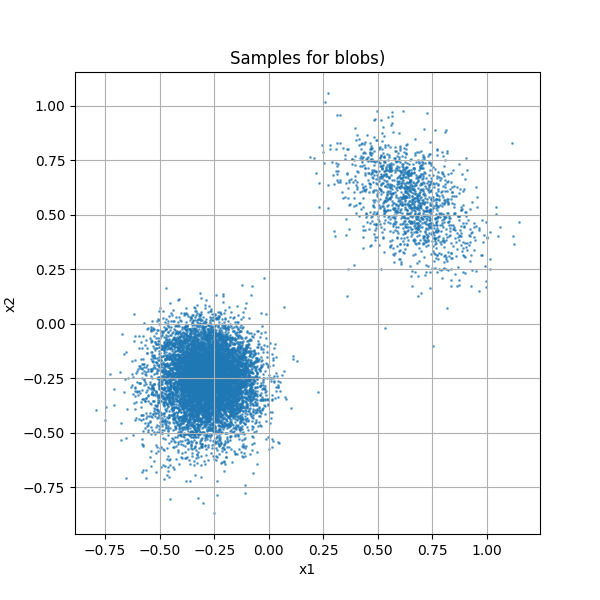
\includegraphics[width=\linewidth]{"images/Samples for ddpm_2_150_0.0001_0.02_blobs.png"}
      \subcaption{Number of time steps = 150}
  \end{minipage}
  \begin{minipage}{0.3\textwidth}
      \centering
      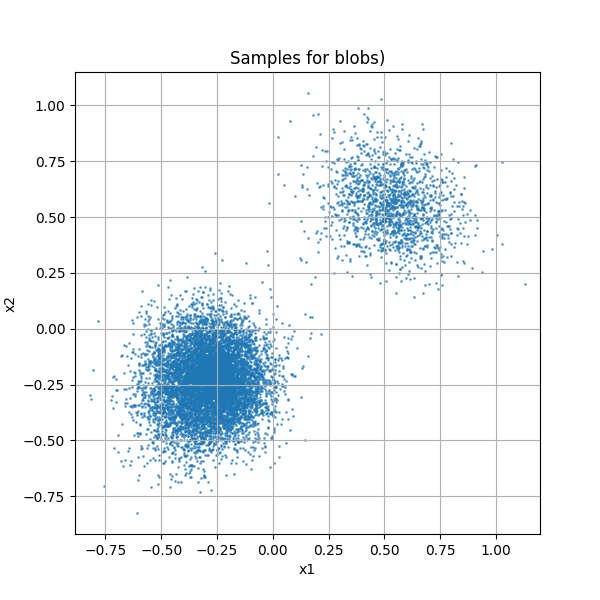
\includegraphics[width=\linewidth]{"images/Samples for ddpm_2_200_0.0001_0.02_blobs.png"}
    \subcaption{Number of time steps = 200}
  \end{minipage}

  \caption{Blobs Dataset}
\end{figure}

Here are the NLL values:
\begin{itemize}
  \item $T = 10$: 0.37
  \item $T = 50$: 0.0152
  \item $T = 100$: 0.0232
  \item $T = 150$: -0.0223
  \item $T = 200$: 0.0045
\end{itemize}

As, we can see from both NLL values and the images, $T = 150$ performed the best. Moreover, there is a sudden decrease in NLL from 10 to 50, which shows the significant impact of increasing the number of time steps.

\clearpage
\subsection*{Many-Circles}

\begin{figure}[H]
  \centering
  \begin{minipage}{0.3\textwidth}
      \centering
      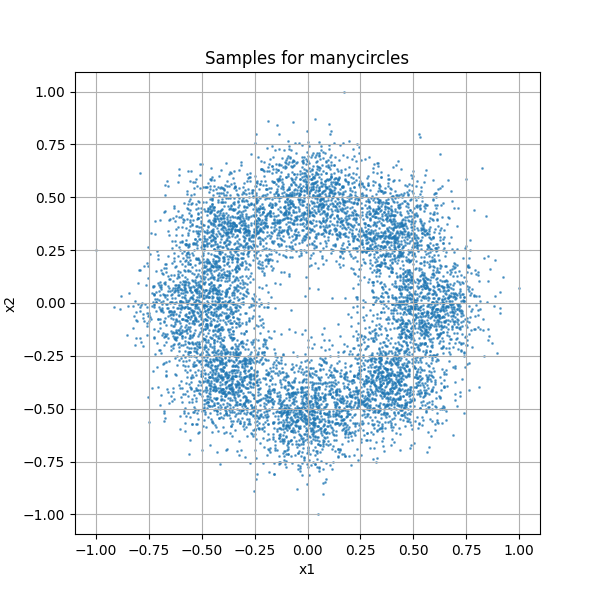
\includegraphics[width=\linewidth]{images/manycircles.png}
      \subcaption{Original ManyCircles Dataset}
  \end{minipage}
  \begin{minipage}{0.3\textwidth}
      \centering
      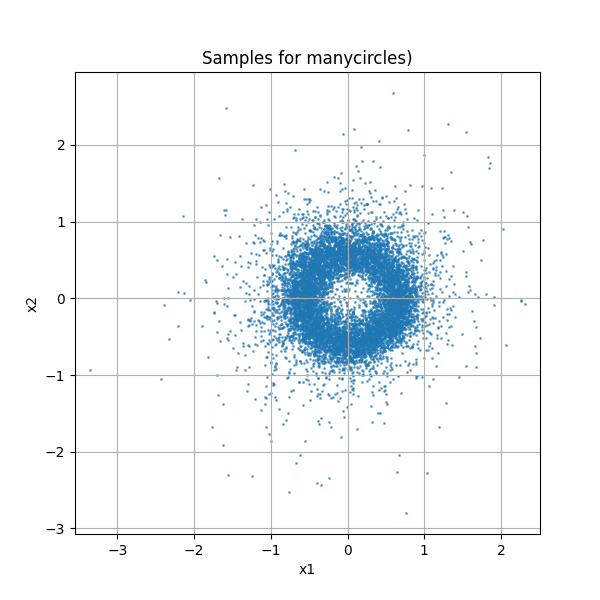
\includegraphics[width=\linewidth]{"images/Samples for ddpm_2_10_0.0001_0.02_manycircles.png"}
      \subcaption{Number of time steps = 10}
  \end{minipage}
  \begin{minipage}{0.3\textwidth}
      \centering
      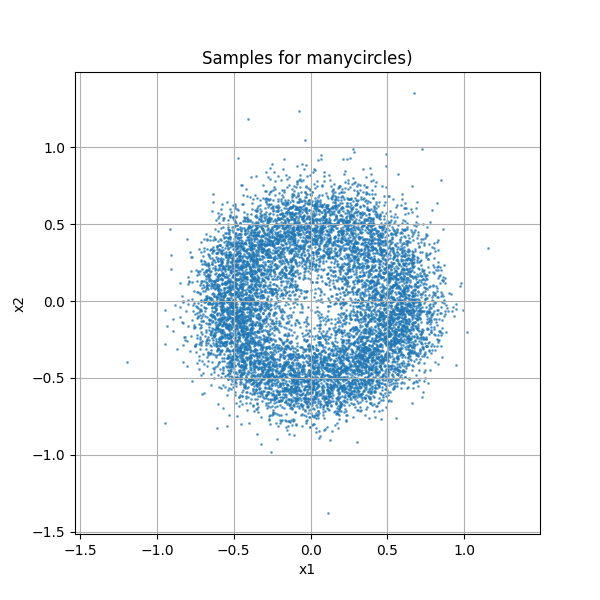
\includegraphics[width=\linewidth]{"images/Samples for ddpm_2_50_0.0001_0.02_manycircles.png"}
      \subcaption{Number of time steps = 50}
  \end{minipage}

  \vspace{0.5cm}

  \begin{minipage}{0.3\textwidth}
      \centering
      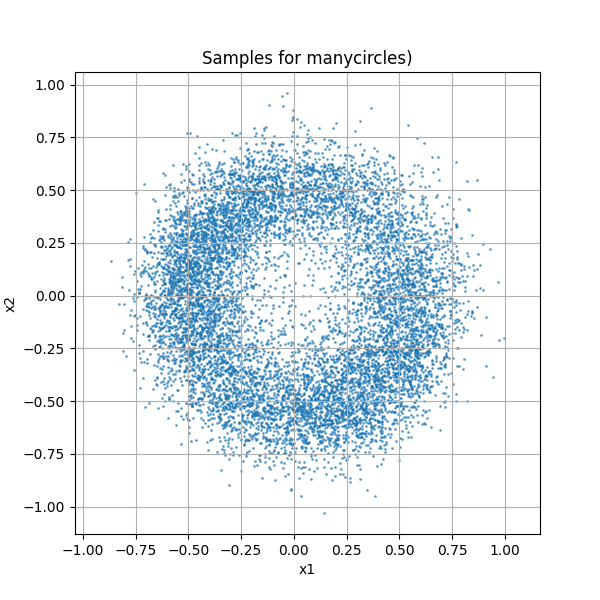
\includegraphics[width=\linewidth]{"images/Samples for ddpm_2_100_0.0001_0.02_manycircles.png"}
      \subcaption{Number of time steps = 100}
  \end{minipage}
  \begin{minipage}{0.3\textwidth}
      \centering
      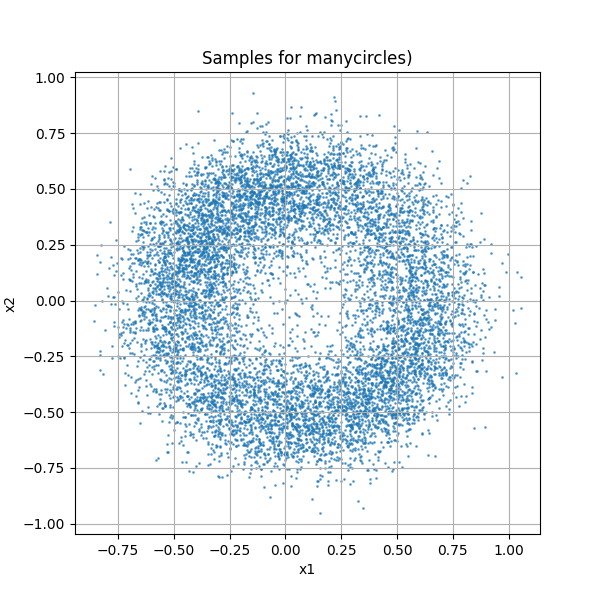
\includegraphics[width=\linewidth]{"images/Samples for ddpm_2_150_0.0001_0.02_manycircles.png"}
      \subcaption{Number of time steps = 150}
  \end{minipage}
  \begin{minipage}{0.3\textwidth}
      \centering
      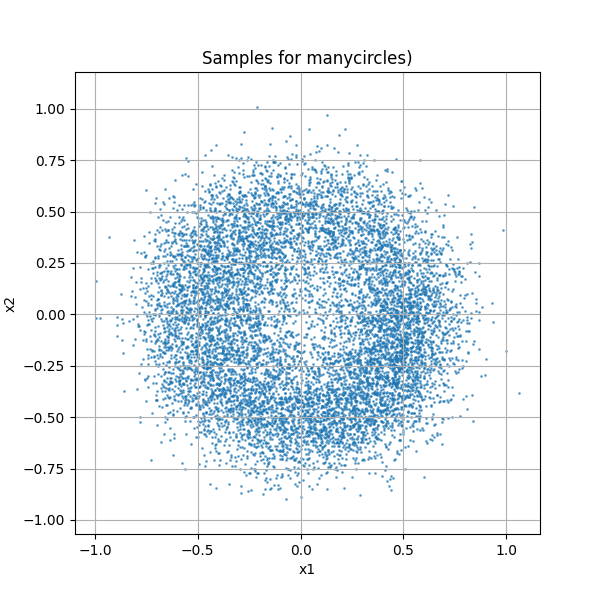
\includegraphics[width=\linewidth]{"images/Samples for ddpm_2_200_0.0001_0.02_manycircles.png"}
    \subcaption{Number of time steps = 200}
  \end{minipage}

  \caption{Many Circles Dataset}
\end{figure}

Here are the NLL values:
\begin{itemize}
  \item $T = 10$: 0.75
  \item $T = 50$: 0.548
  \item $T = 100$: 0.545
  \item $T = 150$: 0.558
  \item $T = 200$: 0.522
\end{itemize}

As, we can see from both NLL values and the images, $T = 200$ performed the best.

\clearpage

\subsection*{Circles}

\begin{figure}[H]
  \centering
  \begin{minipage}{0.3\textwidth}
      \centering
      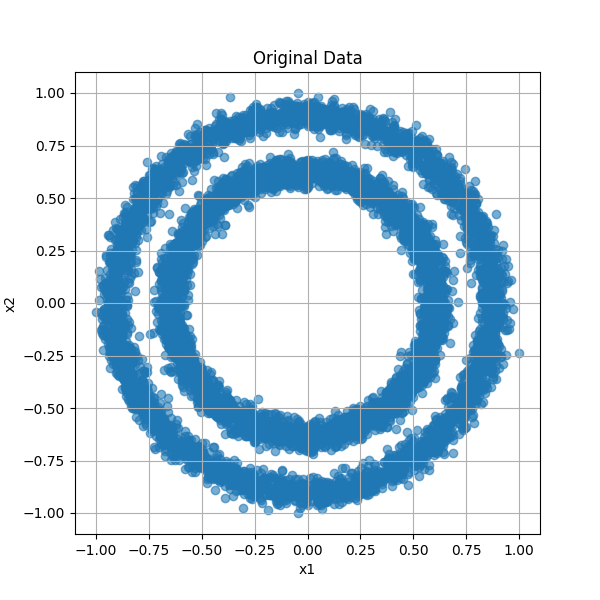
\includegraphics[width=\linewidth]{images/circles.png}
      \subcaption{Original Circles Dataset}
  \end{minipage}
  \begin{minipage}{0.3\textwidth}
      \centering
      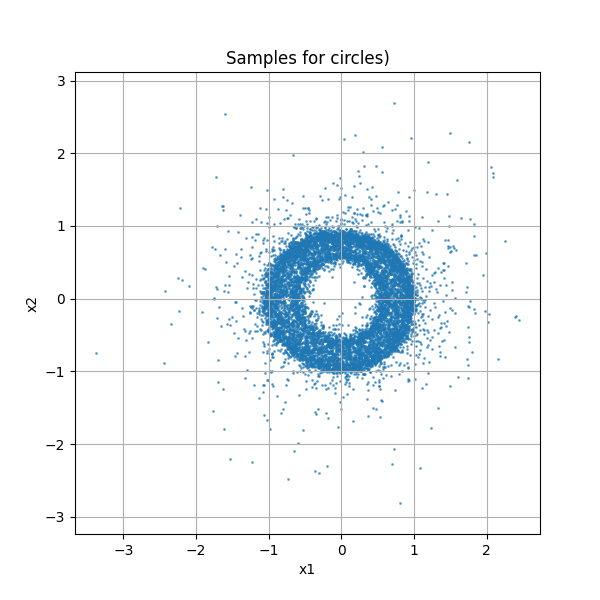
\includegraphics[width=\linewidth]{"images/Samples for ddpm_2_10_0.0001_0.02_circles.png"}
      \subcaption{Number of time steps = 10}
  \end{minipage}
  \begin{minipage}{0.3\textwidth}
      \centering
      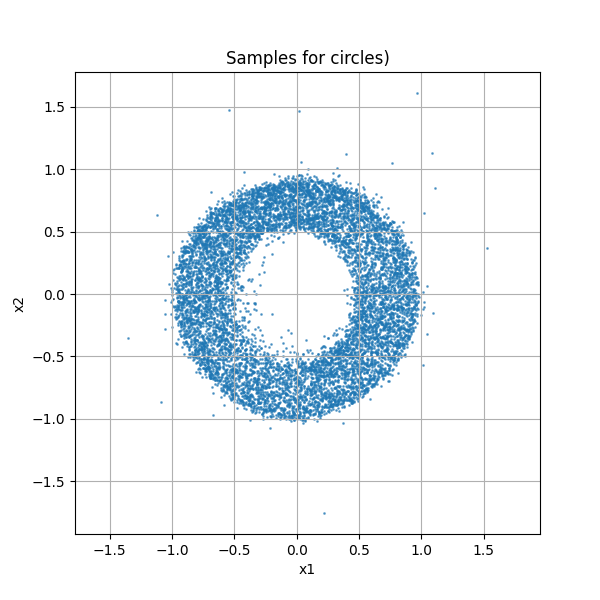
\includegraphics[width=\linewidth]{"images/Samples for ddpm_2_50_0.0001_0.02_circles.png"}
      \subcaption{Number of time steps = 50}
  \end{minipage}

  \vspace{0.5cm}

  \begin{minipage}{0.3\textwidth}
      \centering
      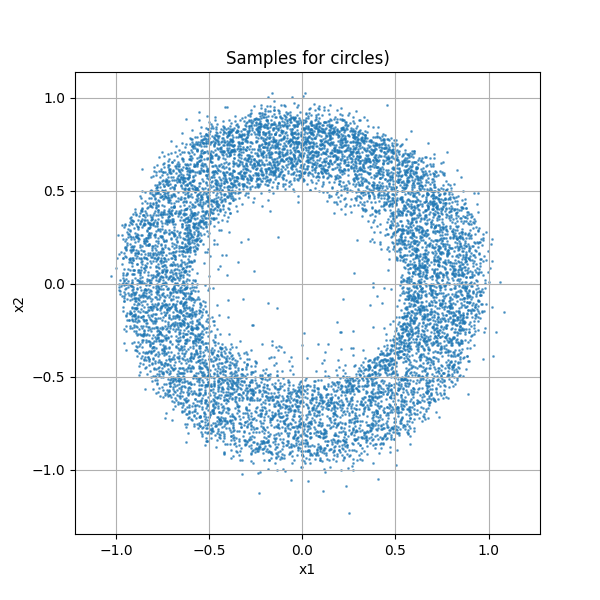
\includegraphics[width=\linewidth]{"images/Samples for ddpm_2_100_0.0001_0.02_circles.png"}
      \subcaption{Number of time steps = 100}
  \end{minipage}
  \begin{minipage}{0.3\textwidth}
      \centering
      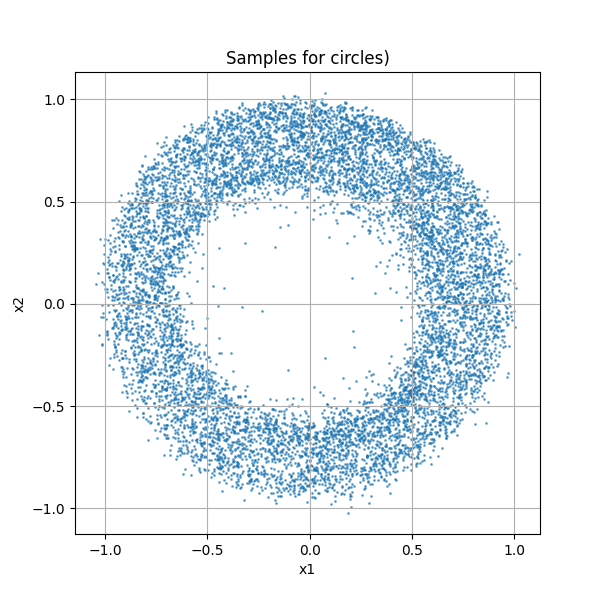
\includegraphics[width=\linewidth]{"images/Samples for ddpm_2_150_0.0001_0.02_circles.png"}
      \subcaption{Number of time steps = 150}
  \end{minipage}
  \begin{minipage}{0.3\textwidth}
      \centering
      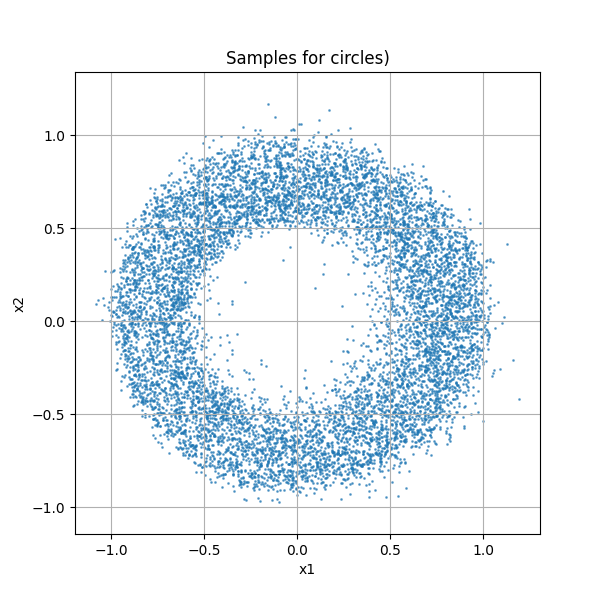
\includegraphics[width=\linewidth]{"images/Samples for ddpm_2_200_0.0001_0.02_circles.png"}
    \subcaption{Number of time steps = 200}
  \end{minipage}

  \caption{Circles Dataset}
\end{figure}


Here are the NLL values:
\begin{itemize}
  \item $T = 10$: 1.081
  \item $T = 50$: 0.991
  \item $T = 100$: 0.9869
  \item $T = 150$: 1.004
  \item $T = 200$: 0.992
\end{itemize}


\clearpage

\subsection*{Helix}

\begin{figure}[H]
  \centering
  \begin{minipage}{0.3\textwidth}
      \centering
      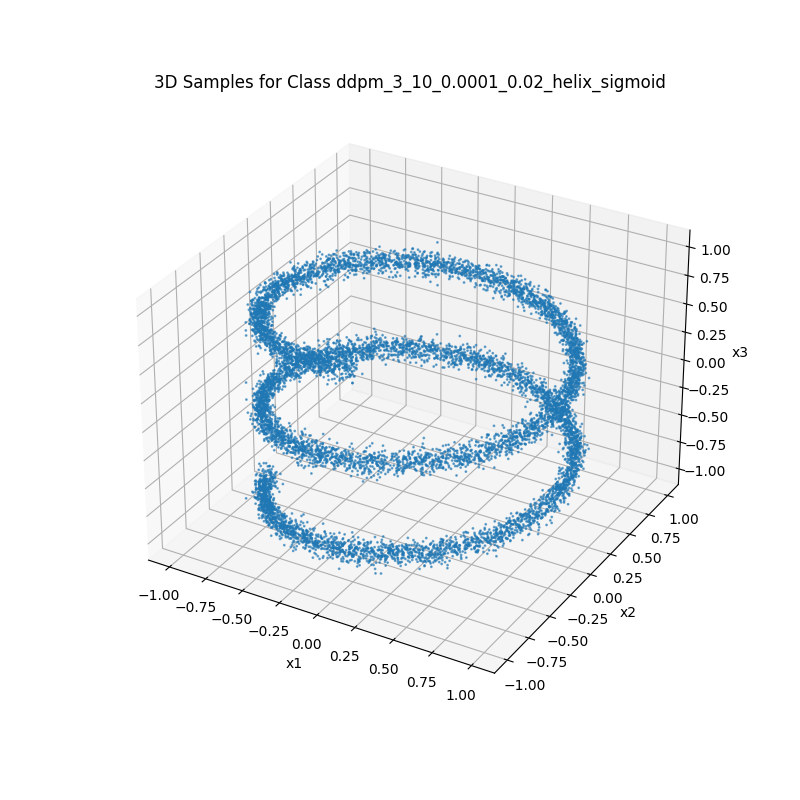
\includegraphics[width=\linewidth]{images/helix.png}
      \subcaption{Original Helix Dataset}
  \end{minipage}
  \begin{minipage}{0.3\textwidth}
      \centering
      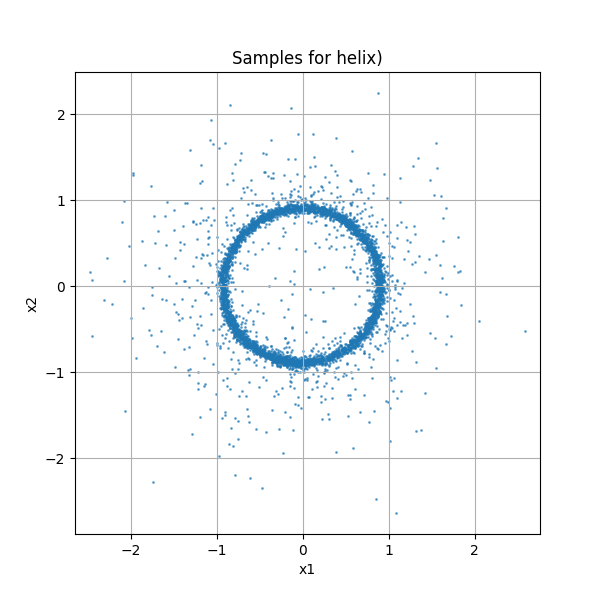
\includegraphics[width=\linewidth]{"images/Samples for ddpm_3_10_0.0001_0.02_helix_sigmoid.png"}
      \subcaption{Number of time steps = 10}
  \end{minipage}
  \begin{minipage}{0.3\textwidth}
      \centering
      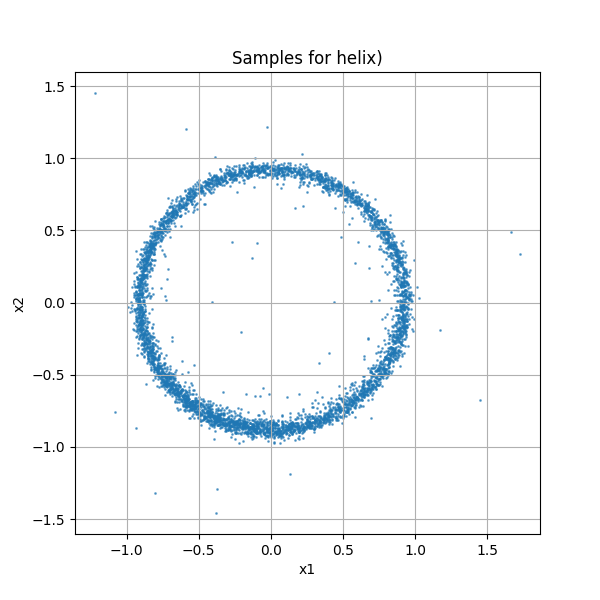
\includegraphics[width=\linewidth]{"images/Samples for ddpm_3_50_0.0001_0.02_helix_sigmoid.png"}
      \subcaption{Number of time steps = 50}
  \end{minipage}

  \vspace{0.5cm}

  \begin{minipage}{0.3\textwidth}
      \centering
      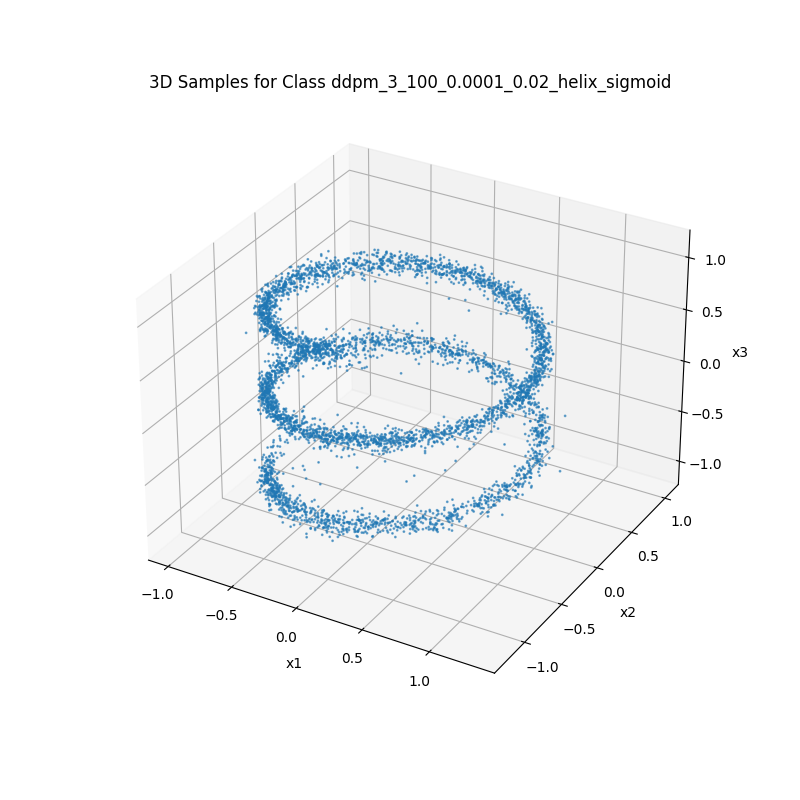
\includegraphics[width=\linewidth]{"images/Samples for ddpm_3_100_0.0001_0.02_helix_sigmoid.png"}
      \subcaption{Number of time steps = 100}
  \end{minipage}
  \begin{minipage}{0.3\textwidth}
      \centering
      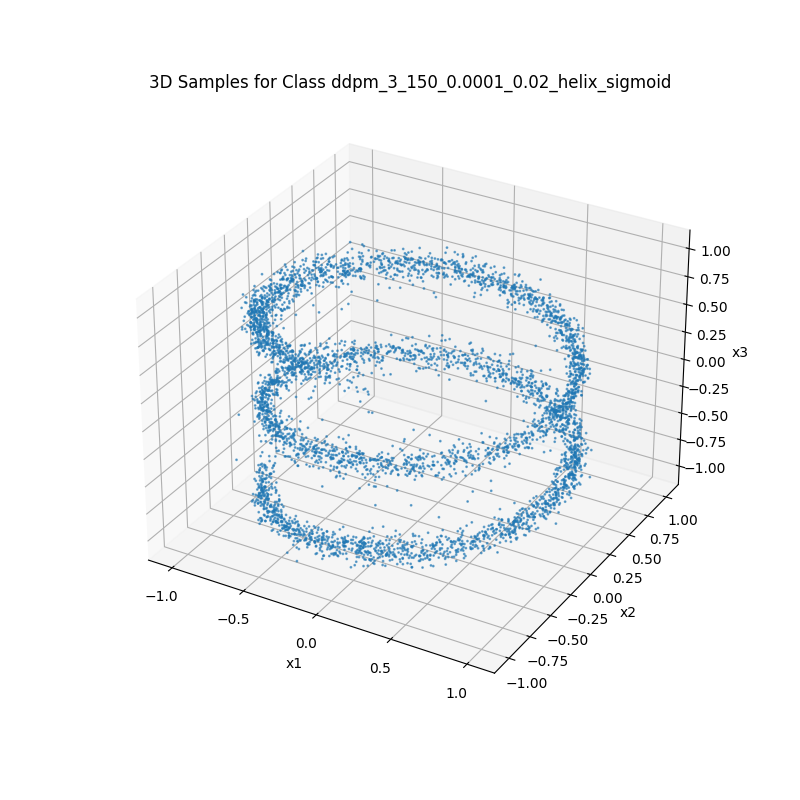
\includegraphics[width=\linewidth]{"images/Samples for ddpm_3_150_0.0001_0.02_helix_sigmoid.png"}
      \subcaption{Number of time steps = 150}
  \end{minipage}
  \begin{minipage}{0.3\textwidth}
      \centering
      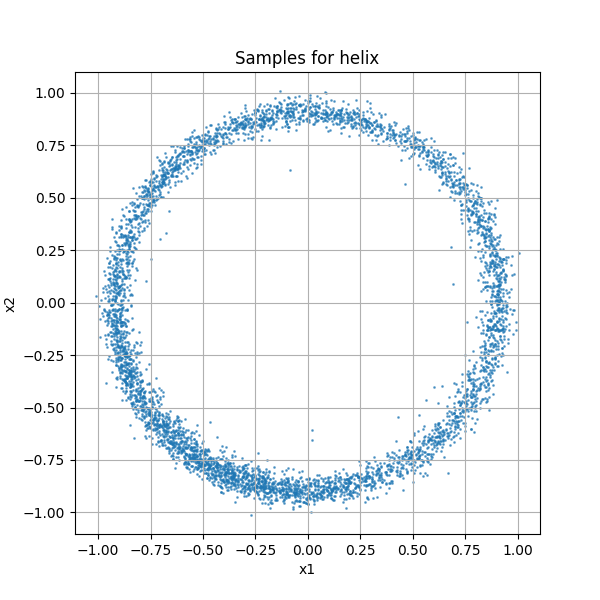
\includegraphics[width=\linewidth]{"images/Samples for ddpm_3_200_0.0001_0.02_helix_sigmoid.png"}
    \subcaption{Number of time steps = 200}
  \end{minipage}

  \caption{Helix Dataset}
\end{figure}


Here are the NLL values:
\begin{itemize}
  \item $T = 10$: 1.6179
  \item $T = 50$: 1.514
  \item $T = 100$: 1.5198
  \item $T = 150$: 1.528
  \item $T = 200$: 1.528
\end{itemize}

As we can see from the images (and the NLL values), 50 performs the best.

\subsection*{Comparison of different noise schedules}
Along with the linear noise schedule, we have studied the effect of cosine and signmoid noise schedules for the DDP model. The results of the comparison are as shown below. In each of the cases we have set the other hyperparameters as follows:
\begin{itemize}
  \item Number of time steps = 200
  \item lbeta=0.0001
  \item ubeta=0.02
  \item lr=0.0001
  \item n\_samples=10000
  \item n\_dim=2
  \item batch\_size=128
  \item epochs=40
\end{itemize}

\subsubsection*{Moons}
\begin{figure}[H]
  \centering
  \begin{minipage}{0.3\textwidth}
      \centering
      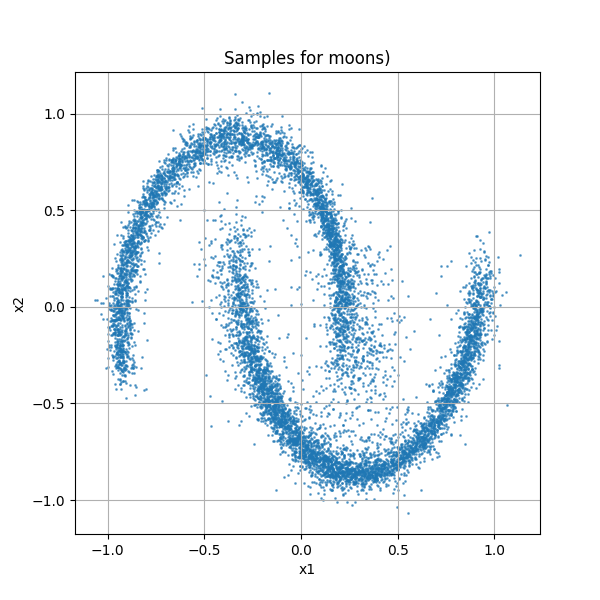
\includegraphics[width=\linewidth]{images/Samples for ddpm_2_200_0.0001_0.02_moons_linear.png}
      \subcaption{Linear Noise Schedule\\NLL=0.932}
  \end{minipage}
  \begin{minipage}{0.3\textwidth}
      \centering
      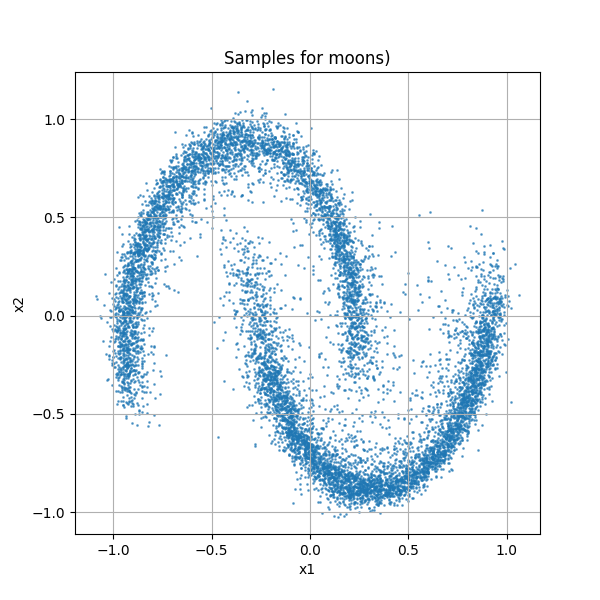
\includegraphics[width=\linewidth]{images/Samples for ddpm_2_200_0.0001_0.02_moons_cosine.png}
      \subcaption{Cosine Noise Schedule\\NLL=0.949}
  \end{minipage}
  \begin{minipage}{0.3\textwidth}
      \centering
      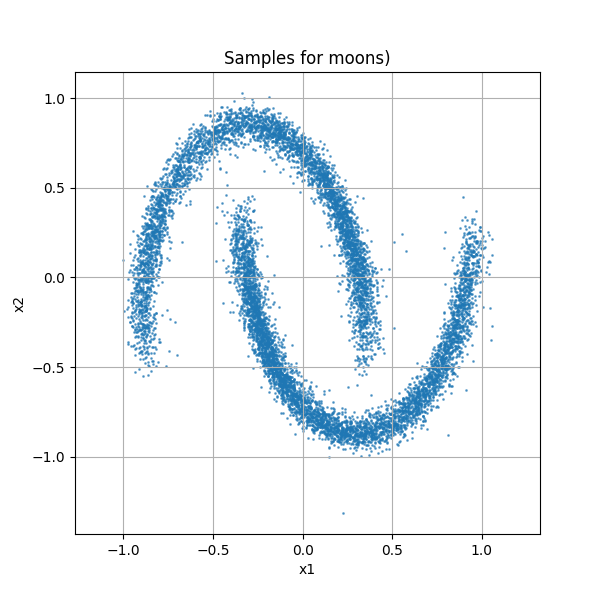
\includegraphics[width=\linewidth]{images/Samples for ddpm_2_200_0.0001_0.02_moons_sigmoid.png}
      \subcaption{Sigmoid Noise Schedule\\NLL=0.928}
  \end{minipage}
\end{figure}
\subsubsection*{Blobs}
\begin{figure}[H]
  \centering
  \begin{minipage}{0.3\textwidth}
      \centering
      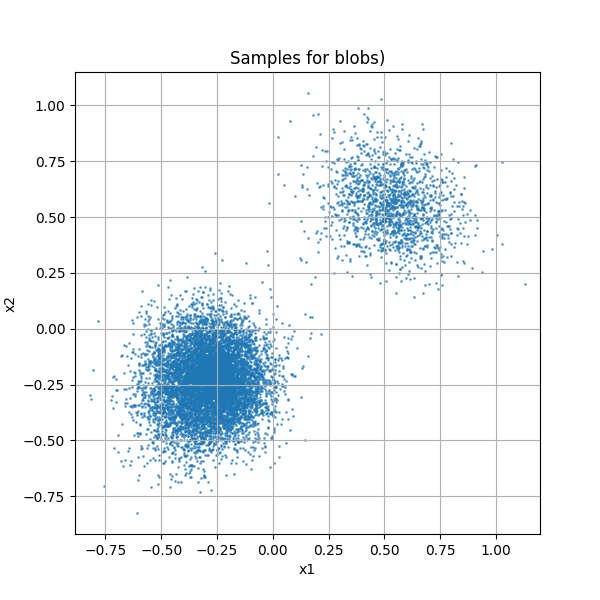
\includegraphics[width=\linewidth]{images/Samples for ddpm_2_200_0.0001_0.02_blobs_linear.png}
      \subcaption{Linear Noise Schedule\\NLL=0.0045}
  \end{minipage}
  \begin{minipage}{0.3\textwidth}
      \centering
      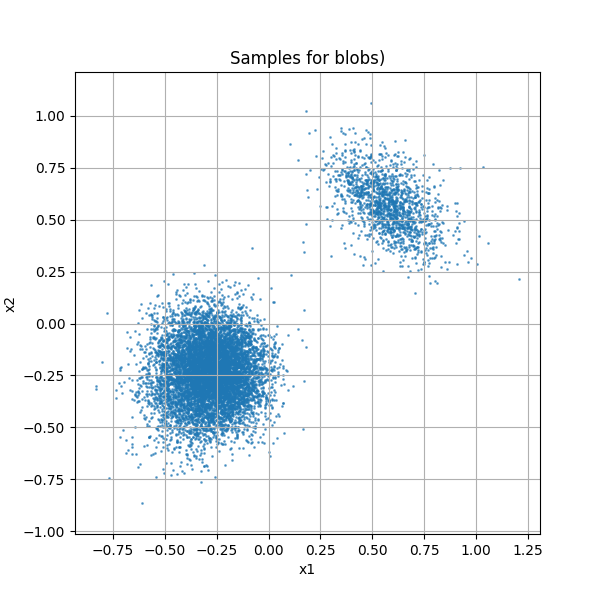
\includegraphics[width=\linewidth]{images/Samples for ddpm_2_200_0.0001_0.02_blobs_cosine.png}
      \subcaption{Cosine Noise Schedule\\NLL=0.0043}
  \end{minipage}
  \begin{minipage}{0.3\textwidth}
      \centering
      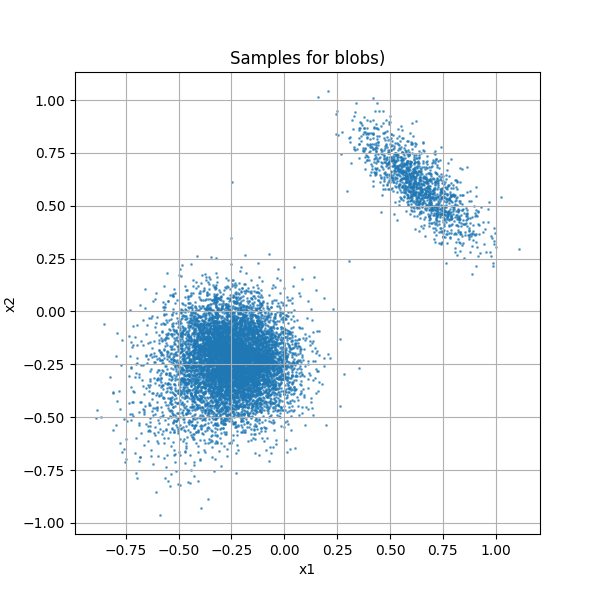
\includegraphics[width=\linewidth]{images/Samples for ddpm_2_200_0.0001_0.02_blobs_sigmoid.png}
      \subcaption{Sigmoid Noise Schedule\\NLL=0.0066}
  \end{minipage}
\end{figure}
In both cases (as well as on the other datasets) we observe that the NLL is least for the sigmoid noise schedule.
\clearpage


\section*{Classifier-Free Guidance}

\subsection*{Difference between Guided Sampling and Conditional Sampling}
In conditional sampling, we model $p(x|y)$ directly, where $y$ is a conditioning variable (like a class label). During generation, we sample from this conditional distribution to get samples that match the condition.

In guided sampling (specifically classifier-free guidance), we train two models: one conditional $p(x|y)$ and one unconditional $p(x)$. During sampling, we interpolate between them with a guidance scale w:
\[\epsilon_\theta(x_t, t, y) = (1+w) * \epsilon_\theta(x_t, t, y) - w * \epsilon_\theta(x_t, t)\]
Firstly, guided sampling is more expensive in terms of computation required to train and sample points (almost double, since we are training two models, and using both of them to sample points). However, this guidance increases the impact of the conditioning information and can produce higher quality samples that better match the condition, but with a potential loss of diversity.

\subsection*{Effect of guidance scale}
We sampled points using CFG on a variety of guidance scale values, here are the images from the moon dataset:

\begin{figure}[H]
  \centering
  \begin{minipage}{0.3\textwidth}
      \centering
      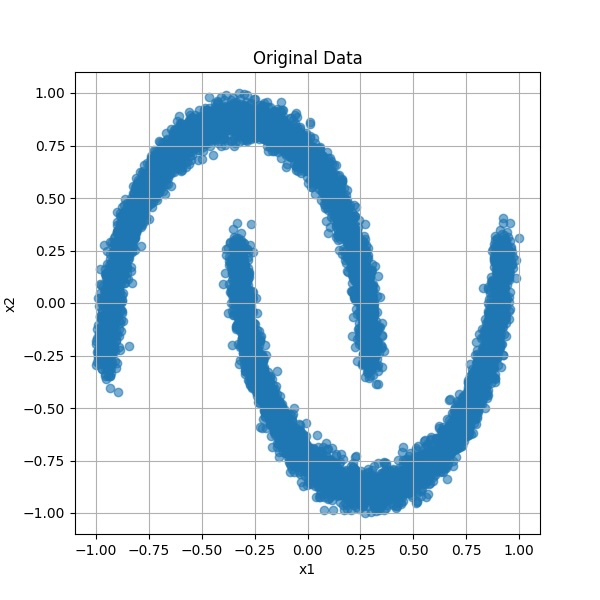
\includegraphics[width=\linewidth]{images/moon.jpg}
      \subcaption{Original Moons Dataset}
  \end{minipage}
  \begin{minipage}{0.3\textwidth}
      \centering
      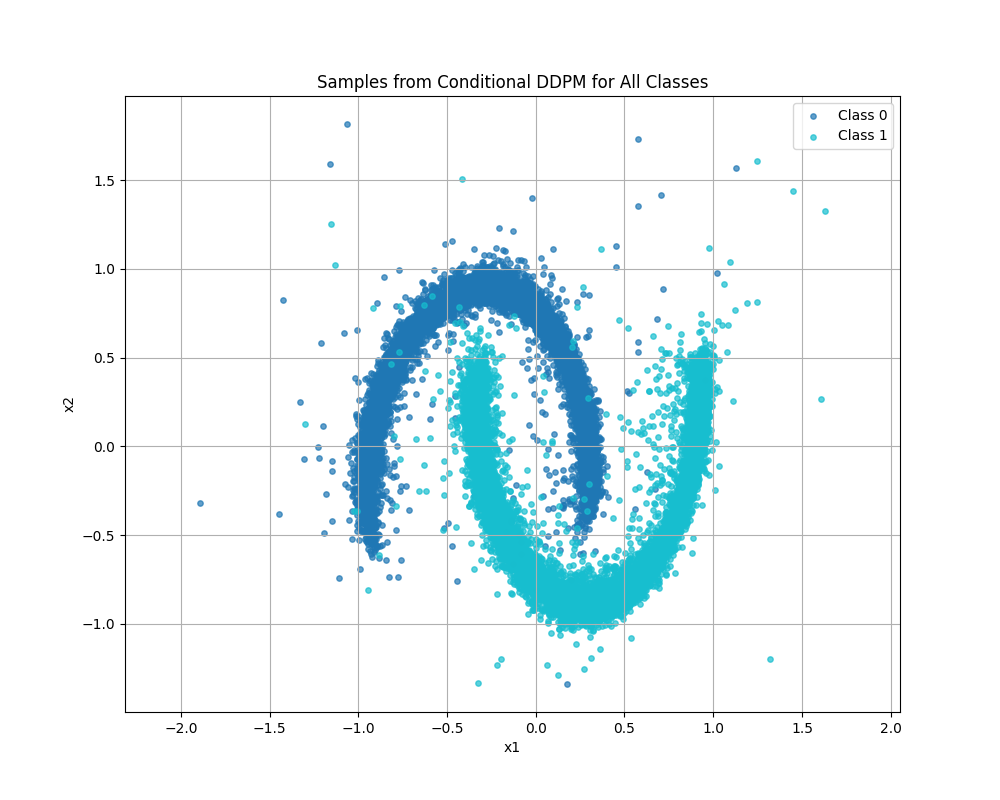
\includegraphics[width=\linewidth]{"images/Samples - CFG for cond_ddpm_2_50_0.0001_0.02_moons_0.0_sigmoid.png"}
      \subcaption{Guidance Scale = 0 (Equivalent to Conditional Sampling)}
  \end{minipage}
  \begin{minipage}{0.3\textwidth}
      \centering
      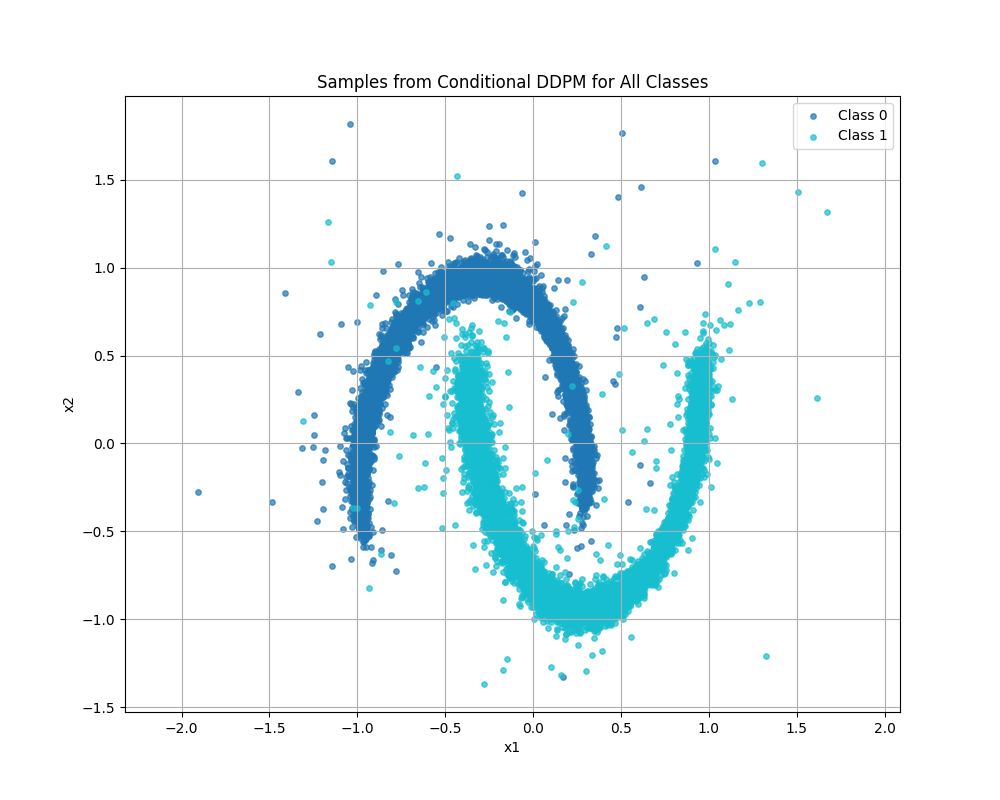
\includegraphics[width=\linewidth]{"images/Samples - CFG for cond_ddpm_2_50_0.0001_0.02_moons_0.2_sigmoid.png"}
      \subcaption{Guidance Scale = 0.2}
  \end{minipage}

  \vspace{0.5cm}

  \begin{minipage}{0.3\textwidth}
      \centering
      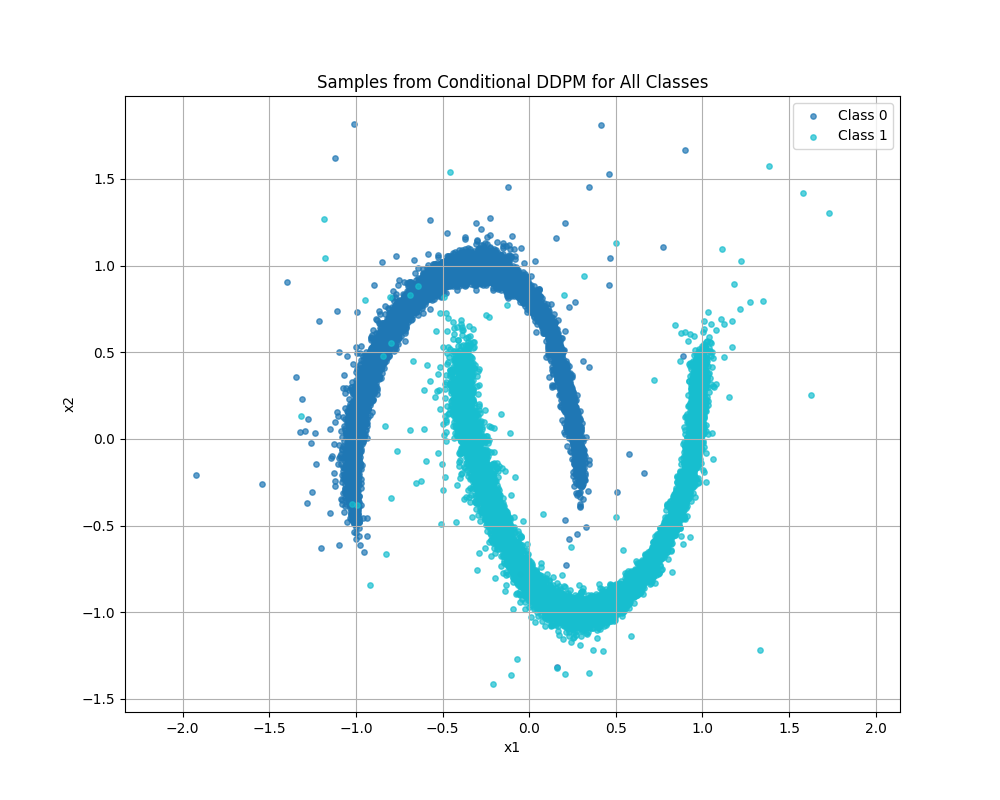
\includegraphics[width=\linewidth]{"images/Samples - CFG for cond_ddpm_2_50_0.0001_0.02_moons_0.5_sigmoid.png"}
      \subcaption{Guidance Scale = 0.5}
  \end{minipage}
  \begin{minipage}{0.3\textwidth}
      \centering
      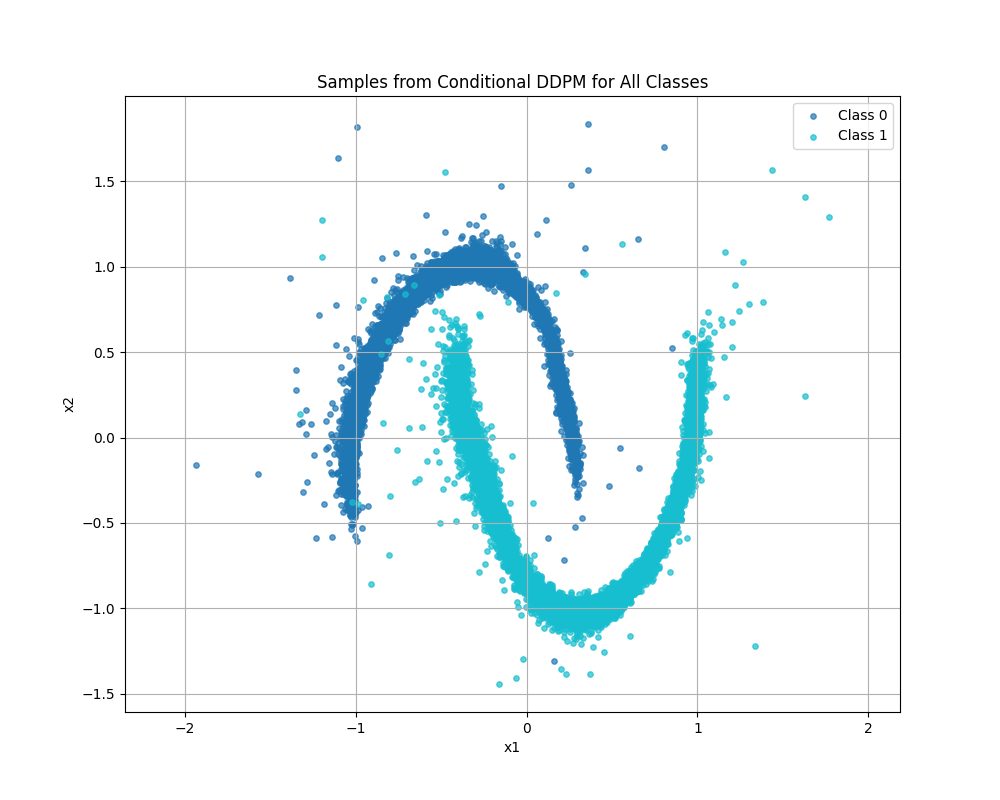
\includegraphics[width=\linewidth]{"images/Samples - CFG for cond_ddpm_2_50_0.0001_0.02_moons_0.7_sigmoid.png"}
      \subcaption{Guidance Scale = 0.7}
  \end{minipage}
  \begin{minipage}{0.3\textwidth}
      \centering
      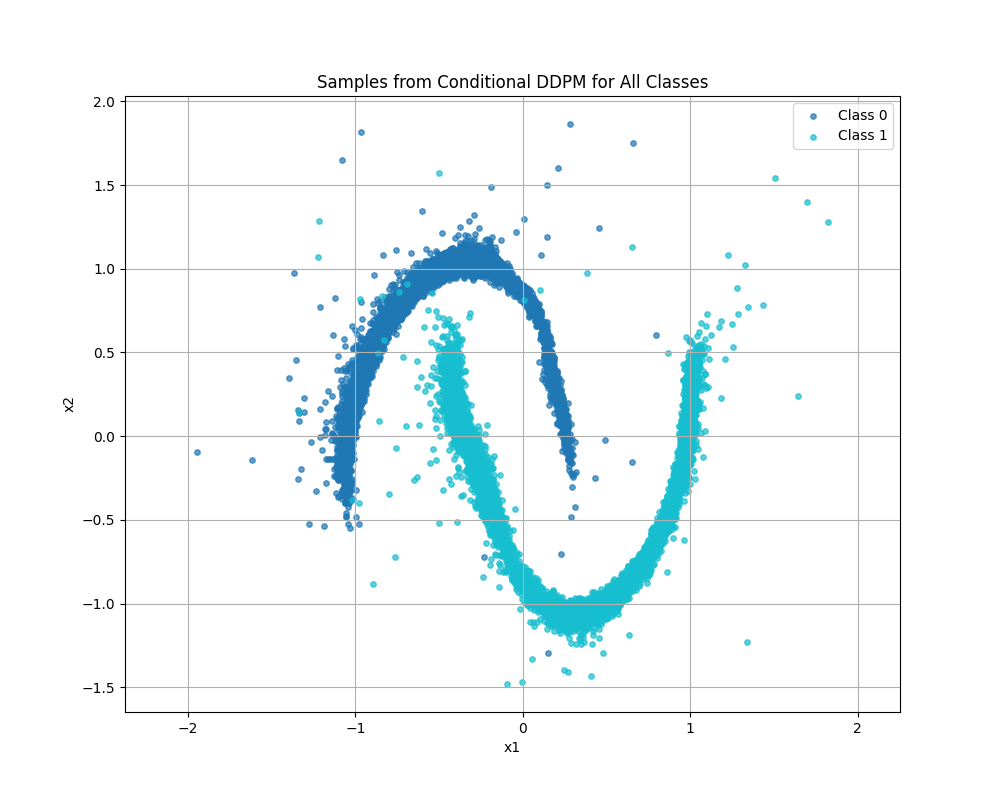
\includegraphics[width=\linewidth]{"images/Samples - CFG for cond_ddpm_2_50_0.0001_0.02_moons_1.0_sigmoid.png"}
    \subcaption{Guidance Scale = 1.0}
  \end{minipage}

  \vspace{0.5cm}

  \begin{minipage}{0.3\textwidth}
      \centering
      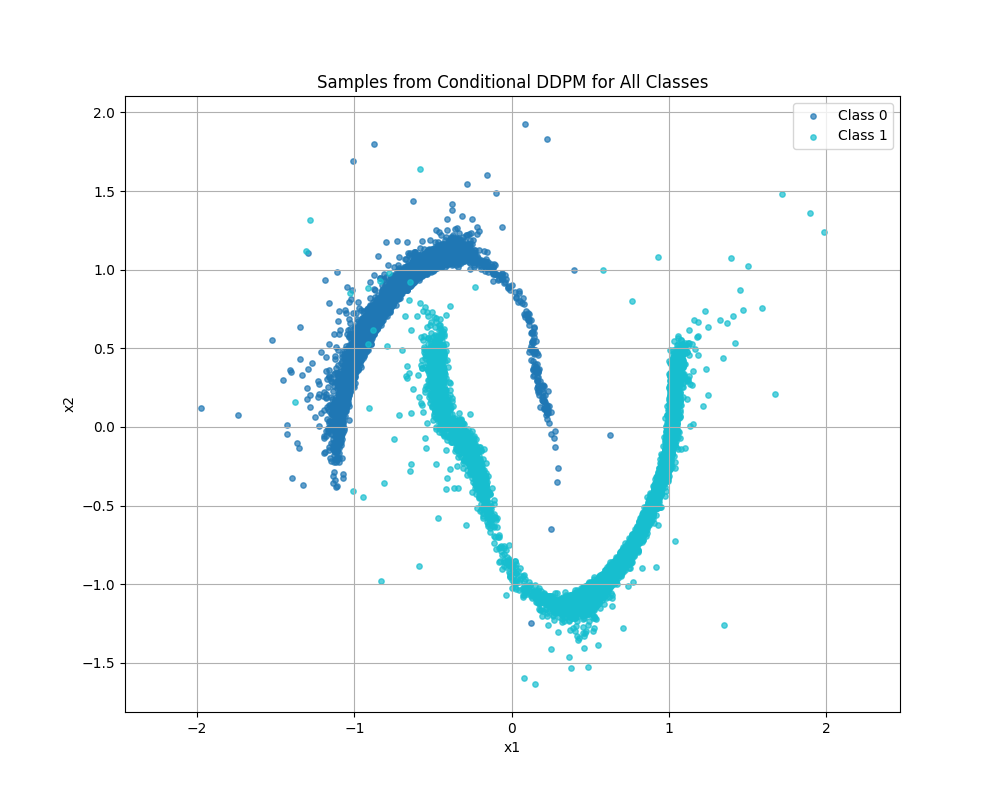
\includegraphics[width=\linewidth]{"images/Samples - CFG for cond_ddpm_2_50_0.0001_0.02_moons_2.0_sigmoid.png"}
      \subcaption{Guidance Scale = 2.0}
  \end{minipage}
  \begin{minipage}{0.3\textwidth}
      \centering
      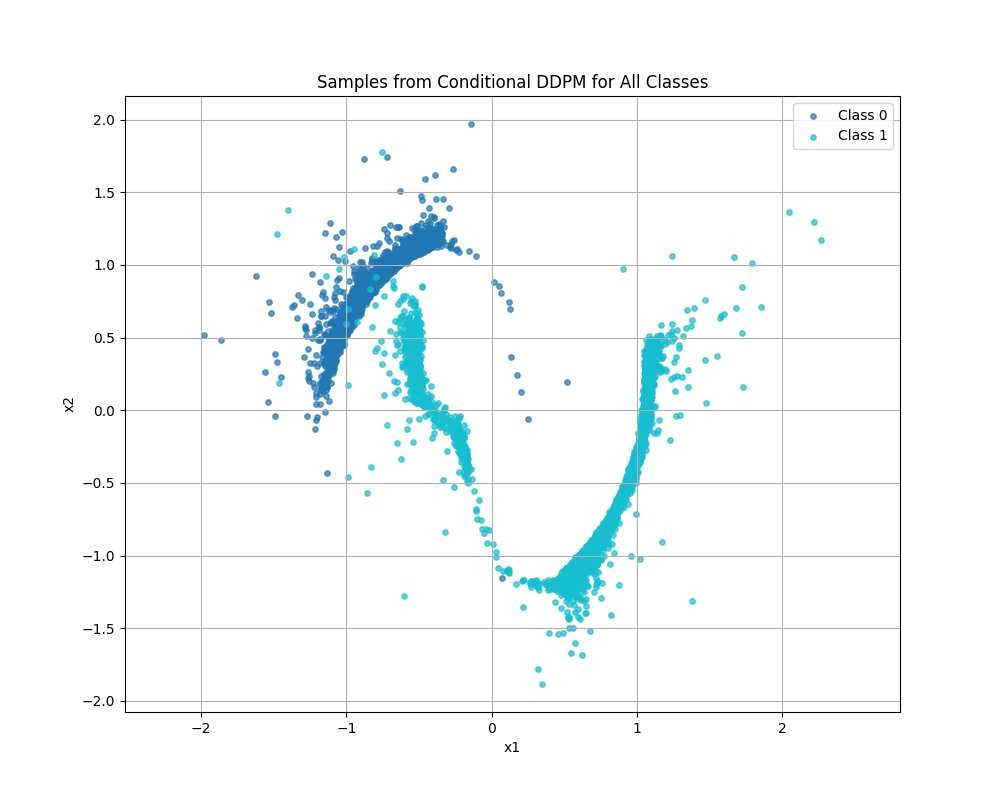
\includegraphics[width=\linewidth]{"images/Samples - CFG for cond_ddpm_2_50_0.0001_0.02_moons_4.0_sigmoid.png"}
      \subcaption{Guidance Scale = 4.0}
  \end{minipage}

  \caption{Moons - CFG}
\end{figure}

\clearpage
\section*{Reward Guidance}





\end{document}
